\documentclass[EU2]{beamer}
% need fontspec for Unicode characters, but don't need font
\usepackage{fontspec}
\usepackage[ngerman]{babel}
\usepackage{csquotes}
\mode<presentation>{\usetheme{Copenhagen}}
\title{Hollerith und die D11}
\author{Simon~Becker, Marek~Kubica}
\date{22.~Mai~2013}
\institute{Technische Universität München}

\hypersetup{pdfencoding=auto}
%\fontspec{Latin Modern Roman}

\beamertemplatenavigationsymbolsempty

% seitenzahlen einfügen
% http://texblog.net/latex-archive/plaintex/beamer-footline-frame-number/
\newcommand*\oldmacro{}%
\let\oldmacro\insertshorttitle%
\renewcommand*\insertshorttitle{%
  \oldmacro\hfill%
  \insertframenumber\,/\,\inserttotalframenumber}

\begin{document}

\frame{\titlepage}

\logo{
\includegraphics[height=1cm]{in_tum}}

\frame{\tableofcontents}

\section{Herman Hollerith}

\subsection{Anfänge}

\begin{frame}{Lebenslauf}
  \begin{columns}
    \column{0.6\textwidth}
    \begin{itemize}
      \item Geboren 29. Februar 1860 in Buffalo, NY
      \item Kind Deutscher Einwanderer
      \item Entwickler von Tabelliermaschienen
      \item Pionier des Einsatzes von Elektrizität
      \item Erfinder (unter anderem Zugbrems-Systeme)
      \item Heirat mit Lu Talcott
      \item Gestorben 17. November 1929
    \end{itemize}
    \column{0.4\textwidth}
      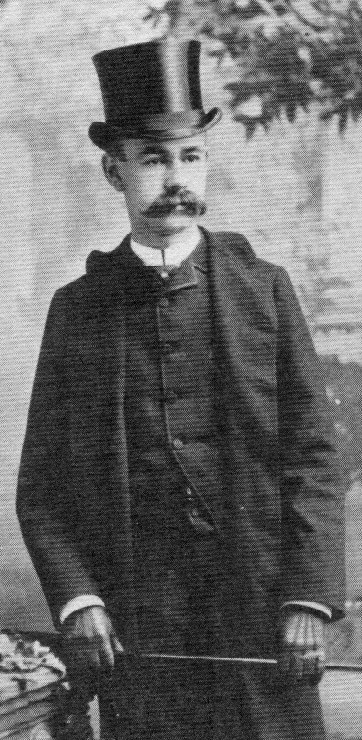
\includegraphics[height=0.8\textheight]{hollerith}\\
      \tiny{Geoffrey D. Austrian, Herman Hollerith — Forgotten Giant of Information Processing}
  \end{columns}
\end{frame}

\subsection{Volkszählungen}

\begin{frame}{1890, USA}
  \begin{itemize}
    \item Vorher in einem Büro der Volkszählung gearbeitet
    \item Ausschreibung für Tabelliersysteme
      \begin{enumerate}
	\item 72~Stunden (Daten) + 5 (Tabellierung) Hollerith
	\item 110 + 44~Stunden Pidgin
	\item 144 + 55~Stunden Hunt
      \end{enumerate}
    \item Innerhalb 6~Wochen verarbeitet
    \item Eine Arbeitskraft verarbeitet 50.000 Personen pro Tag
    \item Gründung von \enquote{The Tabulating Machine Company} in Georgetown
  \end{itemize}
\end{frame}

\begin{frame}[plain]{Bahnticket}
  \begin{center}
    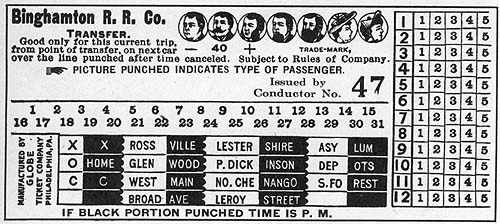
\includegraphics[width=\textwidth]{phototicket}\\
    \tiny{\url{http://discussion.cprr.net/2007/01/punch-photograph-railroad-ticket.html}}
  \end{center}
\end{frame}

\begin{frame}[plain]{Pantograph Punch}
  \begin{center}
    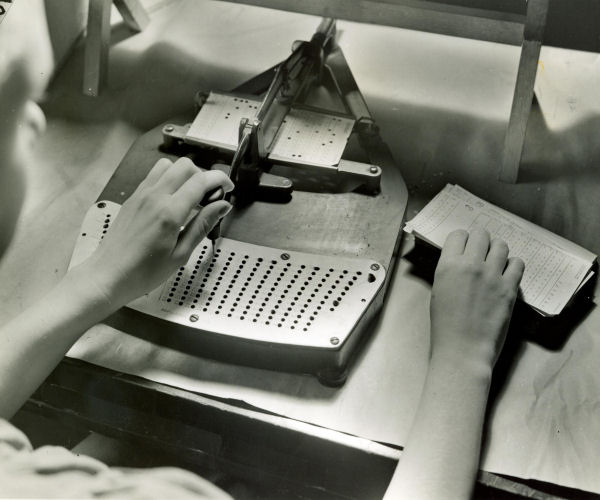
\includegraphics[height=0.9\textheight]{pantograph}\\
    \tiny{\url{https://www.census.gov/history/www/innovations/technology/the\_hollerith\_tabulator.html}}
  \end{center}
\end{frame}

\begin{frame}[plain]{1890er Tabelliermaschine}
  \begin{center}
    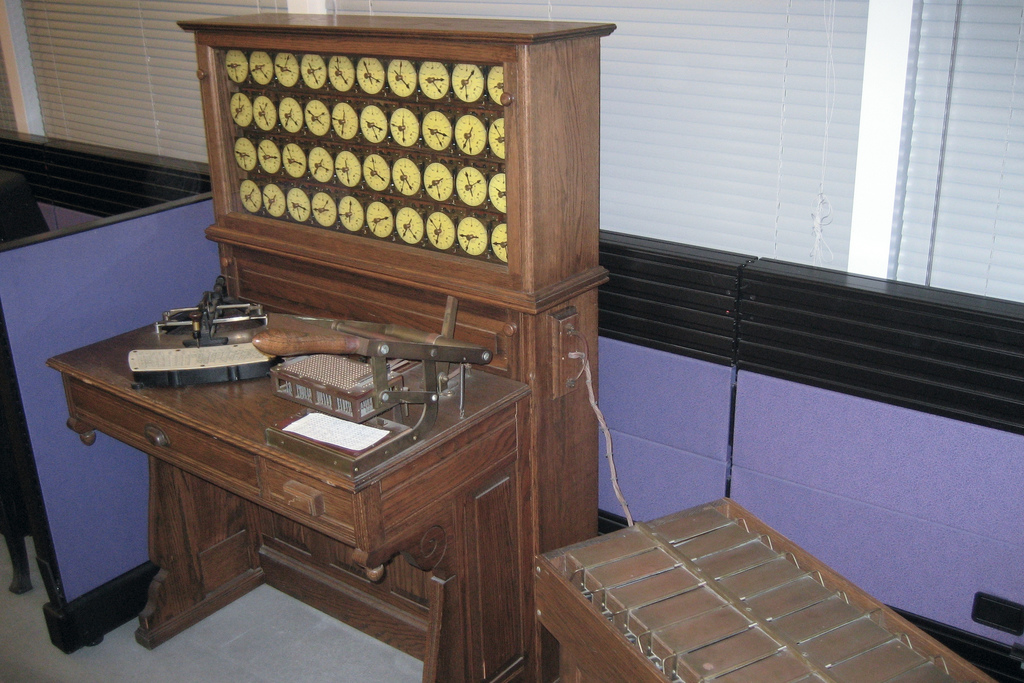
\includegraphics[height=0.9\textheight]{manuell}\\
    \tiny{\url{https://secure.flickr.com/photos/44124384537@N01/411109339}}
  \end{center}
\end{frame}

\begin{frame}{1900, USA}
  \begin{itemize}
    \item TMC wird zur Aktiengesellschaft
    \item Wichtig: Farmstatistiken $\Rightarrow$ Erweiterung der
      Inkrementiermaschinen zu Addiermaschinen
    \item \enquote{Key Punch} Lochstanzmaschine
    \item ab 1901 mit automatischer Sortiermaschine
  \end{itemize}
\end{frame}

\begin{frame}[plain]{Key Punch}
  \begin{center}
    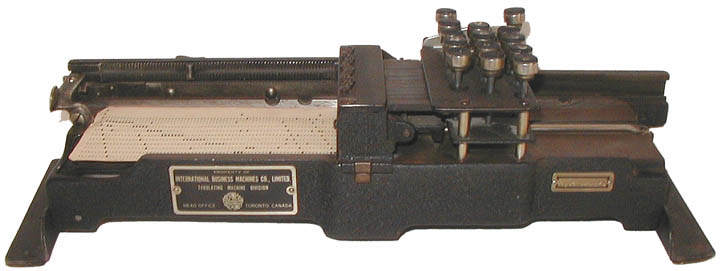
\includegraphics[width=1.09\textwidth]{keypunch}\\
    {\tiny \url{http://www.officemuseum.com/data_processing_machines.htm}}\\
    (Späteres Modell)\\
  \end{center}
\end{frame}

\begin{frame}{Zählungen in anderen Ländern}
  \begin{block}{England}
    \begin{itemize}
      \item Sabotage durch Arbeiter
    \end{itemize}
  \end{block}
  \begin{block}{Österreich}
    \begin{itemize}
      \item Nachbau der Maschinen
    \end{itemize}
  \end{block}
  \begin{block}{Russland}
    \begin{itemize}
      \item Zähe Verhandlungen mit Österreichern und Hollerith
      \item Letztendlich auf Hollerith gesetzt
    \end{itemize}
  \end{block}
  Weitere Länder wie Norwegen, Kanada setzen das System ein.
\end{frame}

\subsection{Kommerzieller Einsatz}

\begin{frame}{Konflikte}
  \begin{block}{Westinghouse}
    Konflikt wegen Bremssystemen für Eisenbahnbremsen, statt hydraulischer
    Signalisierung nutzt Hollerith elektrische, Westinghouse setzt sich jedoch
    zunächst durch.
  \end{block}
  \begin{block}{Österreich}
    Die Österreicher versuchen Holleriths Erfindung selbst zu vermarkten,
    deklarieren Patente für ungültig.
  \end{block}
  \begin{block}{North}
    Organisiert neue Volkszählung, versucht Holleriths Quasi-Monopol zu brechen
    und entwickelt mit Staatsmitteln Tabelliermaschinen (mit Hilfe von James Powers).
  \end{block}
\end{frame}

\begin{frame}{New York Central}
  \begin{itemize}
    \item Eisenbahngesellschaft
    \item Nutzen Holeriths Maschinen schon relativ früh für Buchhaltung
    \item Testballon für komerzielle Vermarktung
  \end{itemize}
  % TODO bild einfügen
\end{frame}

\begin{frame}{Verkauf an C-T-R}
  \begin{itemize}
    \item Charles R. Flint überzeugt Hollerith zu einer Fusion
      \begin{enumerate}
        \item Computing Scale Company
        \item Tabulating Machine Company
	\item International Time Recording Company
	\item Bundy Manufacturing Company
      \end{enumerate}
    \item Neue Firma, Computing Tabulating Recording Company
    \item Thomas J. Watson leitet CTR
    \item CTR wird 1924 zu International Business Machines Corporation, IBM
    \item Hollerith scheidet aus dem Vorstand aus, zeitweise consulting
  \end{itemize}
\end{frame}

\begin{frame}{Geschäftsmodelle}
  \begin{itemize}
    \item Anfangs: Vermietung der Maschinen
    \item Maschinen kostenlos, Lochkarten werden abgerechnet
    \item \enquote{Cloud-Computing}
  \end{itemize}
\end{frame}

\section{DEHOMAG D11}

\begin{frame}[plain]{Dehomag D11 = IBM 450}
  \begin{center}
    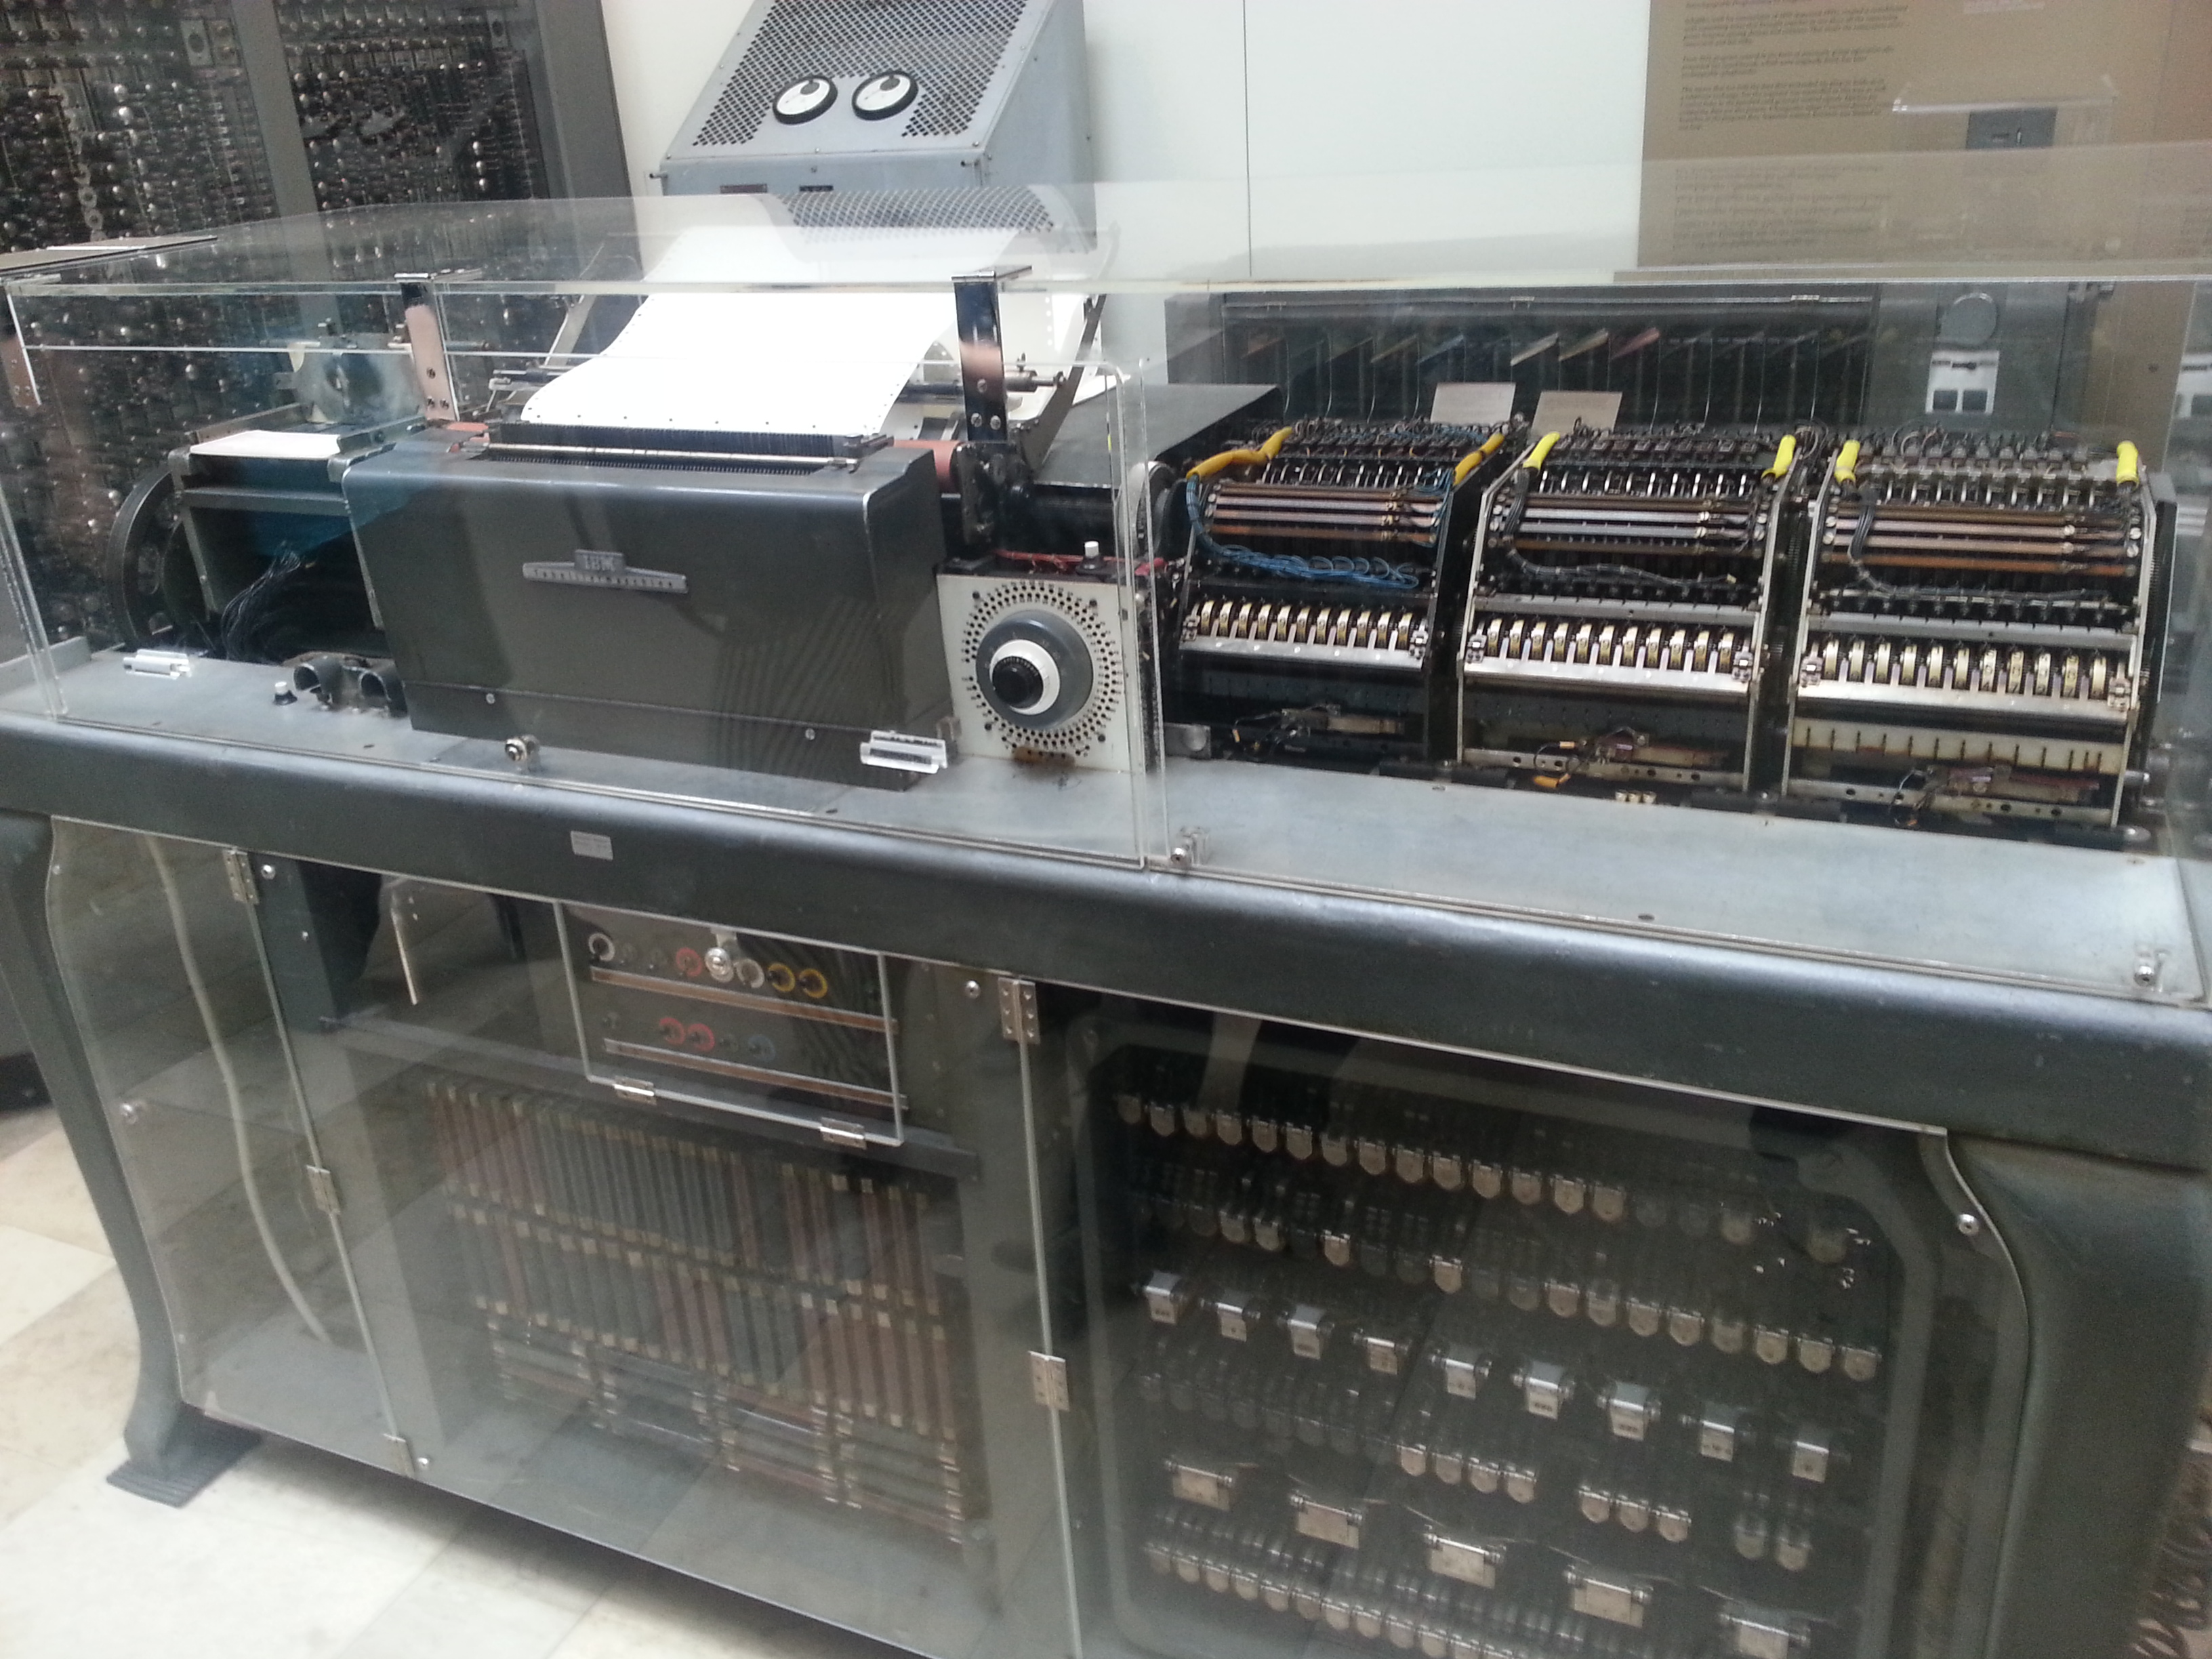
\includegraphics[height=0.95\textheight]{d11}\\
    \tiny{Eigene Aufnahme}
  \end{center}
\end{frame}

\subsection{Bedeutung}

\begin{frame}{D11}
  \begin{itemize}
    \item DEHOMAG, Deutsche Hollerith-Maschinen Gesellschaft mbH
    \item D11 1935 - 1960 in Deutschland gebaut
    \item Erste in großem Maßstab in Deutschland gebaute Maschine
    \item Fabrik in Berlin errichtet
    \item Wir haben eine \emph{funktionsfähige} D11 im Deutschen Museum
  \end{itemize}
  % TODO Bild einfügen
\end{frame}
% Source: Punched-Card Systems and the Early Information Explosion

\subsection{Funktionsweise}

\begin{frame}{Unterschiede zu Holleriths Maschinen}
  \begin{itemize}
    \item Bedruckte Lochkarten
    \item Drucker für Ergebnisse
    \item D11 kann Multiplizieren und Dividieren
  \end{itemize}
\end{frame}

\section{Weiterentwicklung der D11}

\begin{frame}{Kritikpunkte an der D11}
\end{frame}

\begin{frame}{Tabelliermaschine IBM 407}
\end{frame}

\begin{frame}{Tabelliermaschine IBM 421}
\end{frame}

\subsection{Geschichte der Dehomag}
\begin{frame}{…}
\end{frame}

\subsection{Ende der Lochkarte als Speichermedium}
\begin{frame}{…}
\end{frame}

\subsection{Lochkartentechnik heute}
\begin{frame}{…}
\end{frame}

\begin{frame}{Fragen}
  \begin{center}
    \Large{Danke fürs Zuhören!}
  \end{center}
  \begin{center}
    $\vdots$
  \end{center}
  \begin{center}
    \Large{Fragen?}
  \end{center}
\end{frame}

\end{document}

% Volkszählung 1890
% Anfangs Job im Zensusbüro
% Idee zu einer Tabelliermaschiene um die mechanische Arbeit zu verrichten
% Lanston-Kooperation zu Addiermaschienen
% Vortragender am MIT (kurzzeitig), 1882
% Idee die Löcher in Lochkarten für Numerische Werte stehen zu lassen
% Idee der Lochkarten: von punch photographs auf eisenbahnticket
% http://discussion.cprr.net/2007/01/punch-photograph-railroad-ticket.html
% Unterschied zu Jaquard: Elektrizität
% 1884 erstes patent auf Tabelliermaschiene für Volkszählungen
%
% Experimente mit elektrischen Bremssystemen für Züge 1886, 1887, luftbremsen mit elektrosignalisierung statt pneumatik
% erst 1930 wiedererfunden
%
% Karten statt einem langen Band weil einfacher zu lagern, verarbeiten, erstellen
% Robert P. Porter als superindentant für 1890 US Volkszählung
% Ausschreibung für Tabelliermaschienen für 1890
% Konkurenten: Charles F. Pidgin, Mr Hunt
% Neue Punch: pantograph punch
% Testdaten in 72 stunden aufgenommen vs 110 pidgin und 144 hunt
% tabelliermaschiene: 5h statt 44h Pidgin und 55 hunt
%
% Ernstfall: 1890: 50.000 Personen pro Tag gezählt durch eine Arbeitskraft
% Karten unbedruckt, daher einfacher für Maschiene als für Mensch zu lesen
% Auswertung von mehreren werten gleichzeitig durch Relays
% 6 Wochen durchgelaufen
%
% Geschäftsmodell: verleih statt verkauf, weil die Maschienen professionelle Wartung erfordern
%
% Heirat im schnellverfahren mit Lu Talcott
%
% Volkszählung im AUsland: Österreich, Kanada und Norwegen
%
% 1892 Georgetown, "The Tabulating Machine Company"
% Produktion anfangs durch Western Electric (tabul, sorter) und Pratt & Whitney (punch)
% Nach der Volkszählung: alle 105 Tabul wurden zurückgegeben -> fast-pleite
%
% Erweiterung von Inkrementierern auf Addierer -> Accounting
% Feststellung: Besser Tabul konstant an komerzielle Kunden anbieten statt Zensus
%
% Volkszählung in Russland 1895 von Alexander III angeordnet
% Negotiationen mit Hollerith und Österreich wegen Tabulatoren
%
% Einsatz in New York Central (RR)
% Bedruckte Lochkarten mit Separierungsstreifen für Blöcke
% Teilweise wurden die Berechnungen auf die Maschienen in Georgetown ausgelagert
% Ein frühes bespiel von Remote-Computing, Cloud
%
% Tabulating Machine Company, als Aktiengesellschaft
% 1000 Aktien, Hollerith 502
%
% US Volkszählung 1900
% Ausschreibung, Hollerith 185h, Pidgin 452
% Wichtig: Farmstatistiken
% Neue Punch, key punch (einhändige schreibmaschiene)
% Automatic Tabulator (415 karten pro Minute), 80k-90k pro tag
% Lange Zeit keine automatischen sortiermaschienen
% 1901 sortiermaschiene mit 12 taschen
%
% 1901 Tarf-Peirce Company angekauft, die die Tabelliermaschienen bauten
% Anfragen von Retailern 1903
% Tabelliermaschienen kostenlos, alle karten von TMC gekauft und nur für eine bestimmte aufgabe verwendet
%
% Zerwerfung mit North, Zensusdirektor
% North versucht eigene tabelliermaschienen im rahmen des Zensus zu bauen
% 1905 werden Holleriths maschienen aus den Zensusbüro entfernt
%
% Hollerith hört auf mit Zensus, nur noch kommerz
% Kommerzieller Erfolg bei RR
% 1908 Ressourcenknappheit, Lieferverzug
% 1909 wieder im Lot
%
% North baut maschienen, versucht Patente zu umgehen
% Wirbt Holleriths ehemalige mitarbeiter ab
% Mr. Powers, begabter Ingenieur bei North
% Powers punch, erst geschrieben wenn Operator alles absegnet
% Keine Ausschreibung für 1910 Zensus, North muss gehen
%
% Klage gegen Zensusbüro die alten Hollerith-Maschienen umbauen zu wollen
% Gescheitert
% Powers/North-Maschienen langsamer
% Powers geht (später) zu Remington Rand
%
% 1911 zustimmung zu Fusion mit drei anderen Firmen zu CTR:
% Computing-Tabulating-Recording Company aus
% Computing Scale Company of Dayton
% Tabulatimg Machine Company
% International Time Recording Company
% Bundy Manufacturing Company
%
% Hollerith wohlhabend, baut Farm
%
% 1911 CTR fängt an Maschienen selbst zu bauen
%
% 1910 Willy Heidinger interessiert sich für Hollerith's Maschienen
% Deutsche Hollerith Maschienen Gesellschaft, Dehomag
% Lizenzzahlungen an TMC/CTR
% Watson an CTR-Spitze
% Watson lizensiert Hollerith-Patente an Powers/Remington Rand
%
% Hollerith stirbt 17. November 1929
